%-----------------------------------------------------------------------
% Beginning of chap2.tex
%-----------------------------------------------------------------------
%
%  AMS-LaTeX sample file for a chapter of a monograph, to be used with
%  an AMS monograph document class.  This is a data file input by
%  chapter.tex.
%
%  Use this file as a model for a chapter; DO NOT START BY removing its
%  contents and filling in your own text.
% 
%%%%%%%%%%%%%%%%%%%%%%%%%%%%%%%%%%%%%%%%%%%%%%%%%%%%%%%%%%%%%%%%%%%%%%%%


\chapter*{Lecture 15}
\addcontentsline{toc}{chapter}{Lecture 15}
\addtocounter{chapter}{15}
\addtocounter{section}{0}
%\numberwithin{section}{chapter}
\numberwithin{equation}{chapter}
\numberwithin{theorem}{chapter}

%\epigraph{}{--- \textup{}}

In this lecture we study optimality conditions for convex problems of the form

\begin{align*}\label{eq:constr}\tag{1}
\begin{split}
 \minimize & f(\vct{x})\\
 \subjto & \vct{f}(\vct{x})\leq \zerovct\\
         & \vct{h}(\vct{x})= \zerovct,
\end{split}
\end{align*}
where $\vct{x}\in \R^n$, $\vct{f}=(f_1,\dots,f_m)^{\trans}$, $\vct{h}=(h_1,\dots,h_p)$, and the inequalities are componentwise. We assume that $f$ and the $g_i$ are convex, and the $h_j$ are linear. It is also customary to write the conditions $h(\vct{x})=\zerovct$ as $\mtx{A}\vct{x}=\vct{b}$, with $h_j(\vct{x}) = \vct{a}_j^{\trans}\vct{x}-b_j$, $\vct{a}_j$ being the $j$-th row of $\mtx{A}$.

\section{A first-order optimality condition}
So far we have seen two examples of first order optimality conditions: for unconstraint optimization ($\nabla f(\vct{x})=0$) and for linear programming. We now generalize these to the setting of constrained convex optimization.

\begin{theorem}
 Let $f\colon \R^n\to \R$ be a convex, differentiable function, and 
 \begin{equation*}
  \mathcal{F}=\{\vct{x} \mid f_i(\vct{x})\leq 0, \ \mtx{A}\vct{x}=\vct{b}\}
 \end{equation*}
a feasible set, with $f_i$ convex. Then $\vct{x}^*$ is an optimal point of the optimization problem
\begin{equation*}
 \minimize f(\vct{x}) \ \subjto \vct{x}\in \mathcal{F}
\end{equation*}
if and only if for all $\vct{y}\in \mathcal{F}$, 
\begin{equation}\label{eq:opt}
 \ip{\nabla f(\vct{x}^*)}{\vct{y}-\vct{x}^*}\geq 0.
\end{equation}
\end{theorem}

\begin{proof}
 Suppose $\vct{x}^*$ is such that~\eqref{eq:constr} holds. Then, since $f$ is a convex function,
 for all $\vct{y}\in \mathcal{F}$ we have, by Theorem 2.10.1,
 \begin{equation*}
  f(\vct{y})\geq f(\vct{x}^*)+\ip{\nabla f(\vct{x}^*)}{\vct{y}-\vct{x}^*} \geq f(\vct{x}^*),
 \end{equation*}
which shows that $\vct{x}^*$ is a minimizer in $\mathcal{F}$. To show the opposite direction, assume that $\vct{x}^*$ is a minimizer but that~\eqref{eq:constr} does not hold. This means that there exists a $\vct{y}\in \mathcal{F}$ such that $\ip{\nabla f(\vct{x}^*)}{\vct{y}-\vct{x}^*}<0$. Since both $\vct{x}^*$ and $\vct{y}$ are in $\mathcal{F}$ and $\mathcal{F}$ is convex, any point $\vct{z}(\lambda)=(1-\lambda)\vct{x}^*+t\vct{y}$ with $\lambda\in [0,1]$ is also in $\mathcal{F}$. At $\lambda=0$ we have
\begin{equation*}
 \frac{df}{d\lambda}f(\vct{z}(\lambda))|_{\lambda=0} = \ip{\nabla f(\vct{x}^*)}{\vct{y}-\vct{x}^*}<0.
\end{equation*}
Since the derivative at $\lambda=0$ is negative, the function $f(\vct{z}(\lambda))$ is decreasing at $\lambda=0$, and therefore, for small $\lambda>0$, $f(\vct{z}(\lambda))<f(\vct{z}(0))=f(\vct{x}^*)$, in contradiction to the assumption that $\vct{x}^*$ is a minimizer.
\end{proof}

\begin{example}
 In the absence of constraints, $\mathcal{F}=\R^n$, and the statement says that
 \begin{equation*}
  \forall \vct{y}\in \R^n\colon \ip{\nabla f(\vct{x}^*)}{\vct{y}-\vct{x}^*}\geq 0.
 \end{equation*}
If there was a $\vct{y}$ such that $\ip{\nabla f(\vct{x}^*)}{\vct{y}-\vct{x}^*}>0$, then replacing $\vct{y}$ by $2\vct{x}-\vct{y}$ we also have the converse inequality, and therefore the optimality condition is equivalent to saying that $\nabla f(\vct{x}^*)=\zerovct$. We therefore recover the well-known first order optimality condition from Lecture 2. 
\end{example}

Geometrically, the first order optimality condition means that the set
\begin{equation*}
 \{\vct{x}\mid \ip{\nabla f(\vct{x}^*)}{\vct{x}}=\ip{\nabla f(\vct{x}^*)}{\vct{x}^*}\}
\end{equation*}
defines a supporting hyperplane to the set $\mathcal{F}$.

\begin{figure}[h!]
\centering
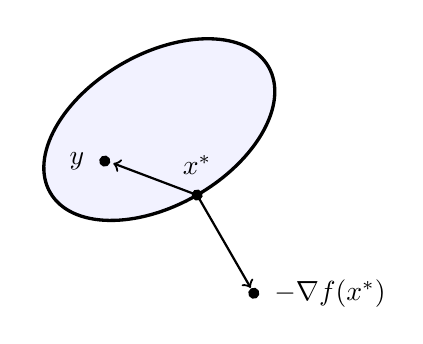
\begin{tikzpicture}[thick,rotate=30,scale=0.8]
\filldraw[color=black, fill=blue!5, very thick](0,0) ellipse (2 and 1.2);
\node (A1) at (0,-3)  [label=0:{$-\nabla f(\vct{x}^*)$}] {};
\node (A2) at (0,-1.2)  [label=90:{$\vct{x}^*$}] {};
%\node (A3) at (0,-2.5)  [label=180:{$\vct{a}$}] {};
\node (A4) at (-1,0)  [label=180:{$\vct{y}$}] {};
\filldraw[black] (0,-3) circle (2pt);
\filldraw[black] (0,-1.2) circle (2pt);
\filldraw[black] (-1,0) circle (2pt);
\draw[color=black, thick, <-] (0,-2.9) -- (0,-1.2);
\draw[color=black, thick, <-] (-0.9,-0.1) -- (0,-1.2);
\end{tikzpicture}
\caption{Optimality condition} \label{fig:neg}
\end{figure}

\section{Lagrangian duality}
Recall the method of Lagrange multipliers. Given two functions $f(x,y)$ and $h(x,y)$, if the problem
\begin{equation*}
 \minimize f(x,y) \quad \subjto h(x,y)=0
\end{equation*}
has a solution $(x^*,y^*)$, then there exists a parameter $\lambda$, the {\em Lagrange multiplier}, such that
\begin{equation}\label{eq:lag}
 \nabla f(x^*,y^*) = \lambda \nabla h(x^*,y^*).
\end{equation}
In other words, if we define the {\em Lagrangian} as 
\begin{equation*}
 \mathcal{L}(x,y,\lambda) = f(x,y)-\lambda h(x,y),
\end{equation*}
then~\eqref{eq:lag} says that $\nabla \mathcal{L}(x^*,y^*,\lambda) = 0$ for some $\lambda$. The intuition is as follows. The set
\begin{equation*}
 M = \{(x,y)\in \R^2 \mid h(x,y)=0\}
\end{equation*}
is a curve in $\R^2$, and the gradient $\nabla h(x,y)$ is perpendicular to $M$ at every point $(x,y)\in M$. For someone living inside $M$, a vector that is perpendicular to $M$ is not visible, it is zero. Therefore the gradient $\nabla f(x,y)$ is zero as viewed from within $M$ if it is perpendicular to $M$, or equivalently, a multiple of $\nabla h(x,y)$.


Alternatively, we can view the graph of $f(x,y)$ in three dimensions. A maximum or minimum of $f(x,y)$ along the curve defined by $h(x,y)=0$ will be a point at which the direction of steepest ascent $\nabla f(x,y)$ is perpendicular to the curve $h(x,y)=0$.

\begin{example}
 Consider the function $f(x,y)=x^2y$ with the constraint $h(x,y)=x^2+y^2-3$ (a circle of radius $\sqrt{3}$). The Lagrangian is the function
 \begin{equation*}
  \mathcal{L}(x,y,\lambda) = x^2y-\lambda(x^2+y^2-3).
 \end{equation*}
Computing the partial derivatives gives the three equations
\begin{align*}
\frac{\partial}{\partial x} \mathcal{L} &= 2xy-2\lambda x = 0\\
\frac{\partial}{\partial y} \mathcal{L} &= x^2-2\lambda y = 0\\
\frac{\partial}{\partial \lambda} \mathcal{L} &= x^2+y^2-3 = 0.
\end{align*}
From the second equation we get $\lambda = \frac{x^2}{2y}$,
and the first and third equations become
\begin{align*}
 2xy-\frac{x^3}{y} &= 0\\
 x^2+y^2-3&=0.
\end{align*}
Solving this system, we get six critical point $(\pm \sqrt{2},\pm 1)$, $(0,\pm \sqrt{2})$. To find out which one of these is the minimizers, we just evaluate the function $f$ on each of these.
\end{example}


We now turn to convex problems of the more general form form
\begin{align}\label{eq:sys1}
\begin{split}
 \minimize & f(\vct{x})\\
 \subjto & \vct{f}(\vct{x})\leq \zerovct\\
         & \vct{h}(\vct{x})= \zerovct,
\end{split}
\end{align}
Denote by $\mathcal{D}$ the {\em domain} of all the functions $f,f_i,h_j$, i.e., 
\begin{equation*}
 \mathcal{D} = \mathrm{dom}(f)\cap \mathrm{dom}(f_1)\cap\cdots\cap\mathrm{dom}(f_m)\cap \mathrm{dom}(h_1)\cap\cdots \cap \mathrm{dom}(h_p).
\end{equation*}
Assume that $\mathcal{D}$ is not empty and let $p^*$ be the optimal value of~\eqref{eq:sys1}.

The {\em Lagrangian} of the system is defined as
\begin{equation*}
 \mathcal{L}(x,y,\lambda) = f(\vct{x})+\vct{\lambda}^{\trans}\vct{f}(\vct{x})+\vct{\mu}^{\trans}h(\vct{x}) = f(\vct{x}) +\sum_{i=1}^m \lambda_i f_i(\vct{x})+\sum_{i=1}^p \mu_i h_i(\vct{x}).
\end{equation*}
The vectors $\vct{\lambda}$ and $\vct{\mu}$ are called the {\em dual variables} or {\em Lagrange multipliers} of the system. The domain of $\mathcal{L}$ is $\mathcal{D}\times \R^m\times \R^{p}$. 

\begin{definition}
 The {\em Lagrange dual} of the problem~\eqref{eq:sys1} is the function
 \begin{equation*}
  g(\vct{\lambda},\vct{\mu}) = \inf_{\vct{x}\in \mathcal{D}} \mathcal{L}(\vct{x},\vct{\lambda},\vct{\mu}).
 \end{equation*}
If the Lagrangian $\mathcal{L}$ is unbounded from below, then the value is $-\infty$.
\end{definition}

The Lagrangian $\mathcal{L}$ is linear in the $\lambda_i$ and $\mu_j$ variables. The infimum of a family of linear functions is concave, so that the Lagrange dual is a concave function. Therefore the negative $-g(\vct{\lambda},\vct{\mu})$ is a convex function.

\begin{lemma}\label{le:lag1}
 For any $\vct{\mu}\in \R^{p}$ and $\vct{\lambda}\geq \zerovct$ we have
 \begin{equation*}
 g(\vct{\lambda},\vct{\mu})\leq p^*.
 \end{equation*}
\end{lemma}

\begin{proof}
 Let $\vct{x}^*$ be a feasible point for~\eqref{eq:sys1}, that is,
 \begin{equation*}
  f_i(\vct{x}^*)\leq 0, \quad h_j(\vct{x}^*)=0,\ 1\leq i\leq m, \ 1\leq j\leq p.
 \end{equation*}
Then for $\vct{\lambda}\geq \zerovct$ and $\mu$, since each $h_j(\vct{x}^*)=0$ and $\lambda_jf_j(\vct{x}^*)\leq 0$, 
\begin{equation*}
 \mathcal{L}(\vct{x}^*,\vct{\lambda},\vct{\mu}) = f(\vct{x}^*)+\sum_{i=1}^m \lambda_if_i(\vct{x}^*)+\sum_{j=1}^p \mu_j h_j(\vct{x}^*)\leq f(\vct{x}^*).
\end{equation*}
In particular,
\begin{equation*}
 g(\vct{\lambda},\vct{\mu}) = \inf_{\vct{x}} \mathcal{L}(\vct{x},\vct{\lambda},\vct{\mu}) \leq \mathcal{L}(\vct{x}^*,\vct{\lambda},\vct{\mu}) \leq f(\vct{x}^*).
\end{equation*}
Since this holds for {\em all} feasible $\vct{x}^*$, it holds in particular for the $\vct{x}^*$ that minimizes~\eqref{eq:sys1}, for which $f(\vct{x}^*)=p^*$. 
\end{proof}

A point $(\vct{\lambda},\vct{\mu})$ with $\vct{\lambda}\geq \zerovct$ and $(\vct{\lambda},\vct{\mu})\in \mathrm{dom}(g)$ is called a {\em feasible point} of the dual problem.

\begin{example}
 Consider a linear programming problem of the form
 \begin{align*}
  \minimize & \ip{\vct{c}}{\vct{x}}\\
  \subjto & \mtx{A}\vct{x}=\vct{b}\\
  & \vct{x}\geq \zerovct.
 \end{align*}
The inequality constraints are $-x_i\leq 0$, while the equality constraints are $\vct{a}_i^{\trans}\vct{x}-b_i$. The Lagrangian has the form
\begin{align*}
 \mathcal{L}(\vct{x},\vct{\lambda},\vct{\mu}) &= \ip{\vct{c}}{\vct{x}}-\sum_{i=1}^n \lambda_i x_i + \sum_{j=1}^m \mu_j(\vct{a}_j^{\trans}\vct{x}-b_j)\\
 &= (\vct{c}-\vct{\lambda}+\mtx{A}^{\trans}\vct{\mu})^{\trans}\vct{x}-\vct{b}^{\trans}\vct{\mu}.
\end{align*}
The infimum over $\vct{x}$ of this function is $-\infty$ unless $\vct{c}-\vct{\lambda}+\mtx{A}^{\trans}\vct{\mu}= \zerovct$. The Lagrange dual is therefore
\begin{equation*}
 g(\vct{\lambda},\vct{\mu}) = \begin{cases} 
                               -\vct{\mu}^{\trans}\vct{b} & \text{ if } \vct{c}-\vct{\lambda}+\mtx{A}^{\trans}\vct{\mu}=\zerovct\\
                               -\infty & \text{ else.}
                              \end{cases}
\end{equation*}
From Lemma~\ref{le:lag1} we conclude that
\begin{equation*}
 \max \{-\vct{b}^{\trans}\vct{\mu} \mid \vct{c}-\vct{\lambda}+\mtx{A}^{\trans}\vct{\mu}=\zerovct, \ \vct{\lambda}\geq \zerovct\} \leq \min \{\vct{c}^{\trans}\vct{x} \mid \mtx{A}\vct{x}=\zerovct, \ \vct{x}\geq \zerovct\}.
\end{equation*}
Note that if we write $\vct{y}=-\vct{\mu}$ and $\vct{s}=\vct{\lambda}$, then we get the dual version of the linear programming problem we started out with, and in this case we know that 
\begin{equation*}
 \max_{\vct{\lambda}\geq \zerovct,\vct{\mu}} g(\vct{\lambda},\vct{\mu}) = p^*.
\end{equation*}
\end{example}

The {\em Lagrange dual} of the optimization problem~\eqref{eq:sys1} is the problem
\begin{equation}\label{eq:lagdual}
 \maximize g(\vct{\lambda},\vct{\mu}) \quad \subjto \vct{\lambda}\geq \zerovct.
\end{equation}
We have seen that if $q^*$ is the optimal value of~\eqref{eq:lagdual}, then $q^*\leq p^*$, and the example above implies that in the special case of linear programming we actually have $q^*=p^*$. We will see that under certain conditions, we have $q^*=p^*$ for more general problems, but this is not always the case.


% %-----------------------------------------------------------------------
% % End of chap1.tex
% %-----------------------------------------------------------------------
